%!TEX root = main.tex

\chapter{Procesos Gaussianos de Regresión}
\label{sec:gaussian}

\begin{chapquote}{Gabriel Lippmann a Henri Poincaré, sobre la distribución gaussiana}
	``Los experimentalistas piensan que es un teorema matemático mientras que los matemáticos creen que es un hecho experimental.''
\end{chapquote}

En los capítulos anteriores definimos todos los elementos necesarios para llegar a definir los procesos gaussianos desde un punto de vista como modelos de regresión. Sin embargo, aún no es claro el por qué de usar estos objectos matemáticos en la tarea de regresión ni como hacerlo. En este capítulo vamos a profundizas en ambas preguntas para responderlas y quede claro la razón del porqué y cómo.

\comment{parrafo: explicando la motivación y por que son importantes, usos, intuición asi como propiedades bonitas}

\comment{parrafo: resumen y guia del capitulo}

\section{Modelos de Regresión}

En las siguientes secciones vamos a hacer una construcción incremental del modelo conocido como una \emph{regresión de procesos gaussianos}. Vamos a partir definiendo el modelo de regresión lineal más simple, para luego ir agregándole complejidad al modelo y deducir así un modelo de regresión no lineal, bayesiano y no paramétrico, coincidiendo con los procesos gaussianos.

\begin{figure}[h]
	\centering
	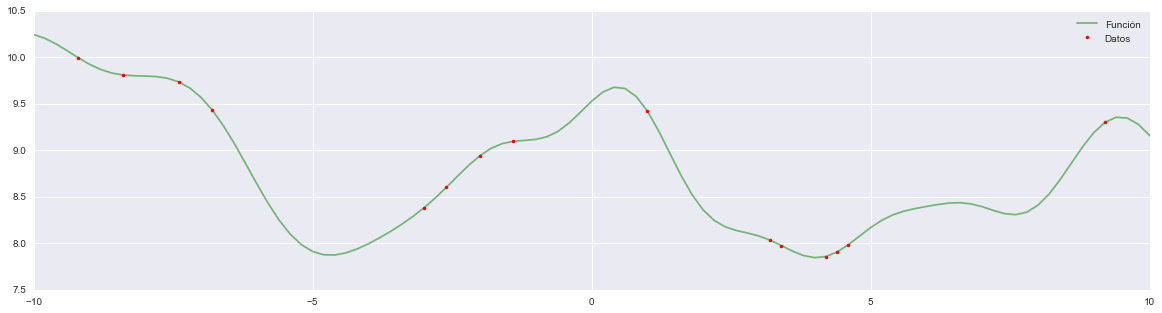
\includegraphics[scale=0.4]{regression}
\end{figure}

Para definir los diferentes modelos de regresión \(f(t) = x\), introduciremos la notación para denotar los conjuntos de datos que serán utilizados en la estimación de los parámetros del modelo. Sea \(\calD = \{(t_i, x_i)\}_{i = 1, \dotsc, n}\) el conjunto de \(n\) pares de datos que se observaron de las variables \((t, x)\), donde \(t = (t^{(1)}, \dotsc, t^{(d)}) \in \calT \subseteq \reals^{1 \times d}\) denota la variable de entrada (variable independiente) e \(x \in \calX \subseteq \reals\) denota la variable de salida (variable dependiente o estado). Denotemos \(T_n = [t_1, \dotsc, t_n]^{\top} \in \reals^{n \times d}\) a la matriz de entrada e \(\bfx_n = [x_1, \dotsc, x_n]^{\top} \in \reals^{n \times 1}\) al vector de salida.

Queremos estimar una función \(f\) a partir de los datos \(\calD_n\), de forma que para todo \(i = 1, \dotsc, n\), los valores \(f(t_i)\) sean cercanos a \(t_i\). Para esto vamos a proponer diferentes formas para \(f\), que dependerá de la base de funciones escogidas y los parámetros. La forma más simple es un modelo lineal, que veremos a continuación.

\subsection{Modelo Lineal}

Consideremos el modelo de regresión lineal simple de parámetros \(w \in \reals^{1 \times d}\) en donde
\begin{equation*}
	x = f(t) = \langle t, w \rangle_{\calT} = t w^{\top}.
\end{equation*}%
Notemos que para agregar una constante al modelo lineal, basta con extender el espacio de entrada en una dimensión, de forma que el modelo lineal es sobre la variable \(\tilde{t} = [1, t]\), por lo que la forma paramétrica del modelo se mantiene intacta.

Si tenemos \(n = d\) datos, donde la matriz cuadrada \(T_n\) es de rango completo, entonces \(w\) y \(f\) se obtienen resolviendo el sistema lineal
\begin{align*}
	T_n w^{\top}	&= \bfx_n,\\
	w^{\top}		&= T_n^{-1} \bfx_n,\\
	f(\bar{t})		&= \bar{t} T_n^{-1} \bfx_n.
\end{align*}%
En general, la cantidad de datos \(n\) no es igual a la dimensión de entrada, por lo que el sistema no tiene solución en el caso general. Un enfoque es estimar el \emph{mejor} modelo lineal posible que se ajuste a los datos, y para esto utilizaremos la técnica conocida como mínimos cuadrados, que se basa en resolver el siguiente problema de optimización:
\begin{equation*}
	\min_{w \in \reals^d} \frac{1}{2} \left\Vert \bfx_n - T_n w^{\top} \right\Vert_n^2.
\end{equation*}

\begin{proposition}
	La solución al problema de mínimos cuadrados lineal tiene solución explícita igual a \(w^{\top} = \left(T_n^{\top} T_n\right)^{-1} T_n^{\top} \bfx_n\), siempre y cuando \(T_n^{\top} T_n\) sea de rango completo.
\end{proposition}

El resultado anterior se obtiene directamente de derivar el funcional a minimizar e igualar el jacobiano a cero:
\begin{align*}
	J(w)									&= \frac{1}{2} \left\Vert \bfx_n - T_n w^{\top} \right\Vert_n^2 = \frac{1}{2} \sum_{i=1}^n \left(x_i - t_i w^{\top}\right)^2,\\
	\dv{J}{w}								&= \sum_{i=1}^n - t_i^{\top} \left(x_i - t_i w^{\top}\right) = 0 \in \reals^d,\\
	\sum_{t=1}^n t_i^{\top} t_i w^{\top}	&= \sum_{i=1}^n t_i^{\top} x_i,\\
	T_n^{\top} T_n w^{\top}					&= T_n^{\top} \bfx_n,\\
	w^{\top}								&= \left(T_n^{\top} T_n\right)^{-1} T_n^{\top}\bfx_n,\\
	f(\bar{t})								&= \bar{t} \left(T_n^{\top} T_n\right)^{-1} T_n^{\top}\bfx_n.
\end{align*}


Podemos ver que si \(T_n\) es invertible, entonces \(n = d\) y se reduce a la expresión anterior. La expresión \(\left(T_n^{\top} T_n\right)^{-1} T_n^{\top}\) se conoce como la pseudoinversa de Moore-Penrose de \(T_n\), y se denota como \(T_n^+\), de forma de que la solución se puede reescribir como \(f(\bar{t}) = \bar{t} T_n^+ \bfx_n\). 

\subsection{Modelo Lineal con Ruido}
Consideremos el caso que la variable \(x\) tiene ruido \(\varepsilon\) generado de una fuente aleatoria:
\begin{equation*}
	x = t w^{\top} + \varepsilon.
\end{equation*}%

\begin{figure}[h]
	\centering
	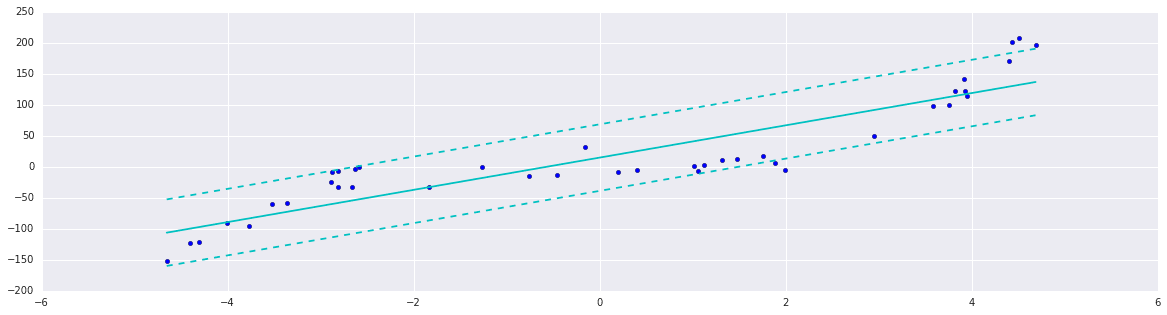
\includegraphics[scale=0.4]{linear}
\end{figure}

Si suponemos que los ruidos (o errores) son independientes e idénticamente distribuidos de forma normal, entonces podemos escribir el modelo de forma que
\begin{align*}
	x_i				&= t_i w^{\top} + \varepsilon_i,\\
	\varepsilon_i	&\sim \calN \left(0, \sigma^2\right),\\
	x \mid t		&\sim \calN \left(t w^{\top}, \sigma^2\right),
\end{align*}
donde \(\sigma^2\) es el parámetro de ruido del modelo. Queremos estimar los parámetros \(w\) y \(\sigma^2\), de modo que el modelo generado sea lo más verosímil posible. La noción de verosimilitud del modelo será modelada como la probabilidad de que los datos hayan sido generadas por el modelo parámetro, es decir,
\begin{equation*}
	\calL \left(w, \sigma^2\right) = p\left(\bfx_n \mid T_n, w, \sigma^2\right),
\end{equation*}
la cual en el caso gaussiano independiente se tiene de forma explícita:
\begin{align*}
	\calL \left(w, \sigma^2\right)	&= \prod_{i=1}^n p\left(x_i \mid t_i, w, \sigma^2\right)\\
									&= \frac{1}{(2\pi)^{\frac{n}{2}} \sigma^n} \exp \left(-\frac{1}{2\sigma^2} \sum_{i=1}^n \left(x_i - t_i w^{\top}\right)^2\right).
\end{align*}

Para maximizar la verosimilitud, podemos aplicar logaritmo a la función objetivo, y si cambiamos el signo entonces tenemos la función de log-verosimilitud negativa, denotada NLL por las siglas en inglés de \emph{negative log-likelihood}, la cual debemos minimizar:
\begin{equation*}
	\ell \left(w, \sigma^2\right) = \frac{n}{2} \ln(2\pi) + n \ln(\sigma) + \frac{1}{2\sigma^2} \sum_{i=1}^n \left(x_i - t_i w^{\top}\right)^2.
\end{equation*}
Podemos ver que la función a minimizar es similar al caso no probabilista, pero con el parámetro \(\sigma\) adicional. Derivando con respecto a los parámetros \(w\) y \(\sigma\) para luego igualar a cero, se obtiene que
\begin{align*}
	\dv{\ell}{w}		&= \frac{1}{\sigma^2} \sum_{i=1}^n - t_i^{\top} \left(x_i - t_i w^{\top}\right) = 0,\\
						&\implies w^{\top} = \left(T_n^{\top} T_n\right)^{-1} T_n^{\top}\bfx_n,\\
	\dv{\ell}{\sigma}	&= \frac{n}{\sigma} - \frac{1}{\sigma^3} \sum_{i=1}^n \left(x_i - t_i w^{\top}\right)^2 = 0,\\
						&\implies \sigma^2 = \frac{1}{n} \sum_{i=1}^n \left(x_i - t_i w^{\top}\right)^2,
\end{align*}
luego la probabilidad predictiva de \(f(x)\) es
\begin{align*}
	p\left(\bar{f} \mid \bar{t}, T_n, \bfx_n\right)	&= \calN \left(\bar{\mu}_{\bar{f}}, \bar{\sigma}_{\bar{f}}^2\right),\\
	\bar{\mu}_{\bar{f}}								&= \bar{t} \left(T_n^{\top} T_n\right)^{-1} T_n^{\top} \bfx_n,\\
	\bar{\sigma}_{\bar{f}}^2						&= \frac{1}{n} \left\Vert \bfx_n - T_n w^{\top} \right\Vert_n^2.
\end{align*}
Podemos ver que los parámetros \(w\) coinciden con el caso no probabilista, pero nos entrega una medida de la varianza del ruido, que coincide con el error cuadrático promedio.

\subsection{Modelo Lineal Bayesiano}

Siguiendo el formalismo bayesiano, es necesario especificar una distribución \emph{a priori} sobre los parámetros \(w\). Consideremos el caso en el que los pesos se distribuyen \emph{a priori} de forma normal con media nula y matriz de covarianza \(\Sigma_{w}\):
\begin{equation*}
	w \sim \calN \left(0, \Sigma_w\right).
\end{equation*}%
Podemos aplicar el Teorema de Bayes para encontrar la distribución \emph{a posteriori} de \(w\) dado los datos observados:
\begin{equation*}
	p(w \mid T_n, \bfx_n) = \frac{p(\bfx_n \mid T_n, w) p(w)}{p(\bfx_n \mid T_n)}.
\end{equation*}
Se puede ver que la función a minimizar es la suma entre la NLL y la log-prior negativa (NLP), la cual en un enfoque no bayesiano se considera como un termino de penalización:
\begin{equation*}
	NLP = \frac{d}{2} \ln(2\pi) + d \ln \left\vert \Sigma_w \right\vert + \frac{1}{2} w \Sigma_w^{-1} w.
\end{equation*}
Si combinamos la distribución a priori \(p(w) = \calN (0, \Sigma_w)\) con la verosimilitud de los parámetros \(p(\bfx_n \mid T_n, w) = \calN \left(T_n w^{\top}, \sigma^2 I_n\right)\) de forma analítica, obtenemos que la distribución a posteriori de \(w\) es normal:
\begin{align*}
	w \mid T_n, \bfx_n	&\sim \calN\left(\Sigma_w^{T_n} T_n^{\top} \bfx_n, \sigma^2 \Sigma_w^{T_n}\right),\\
	\Sigma_w^{T_n}		&= \left(T_n^{\top} T_n + \sigma^2 \Sigma_w^{-1}\right)^{-1}.
\end{align*}
Como su media y su moda coinciden, el estimador máximo a posteriori de \(w\) (denotado MAP por sus siglas en inglés \emph{maximum a posteriori}) es igual a
\begin{align*}
	\hat{w}	&= \Sigma_w^{T_n} T_n^{\top} \bfx_n,\\
			&= \left(T_n^{\top} T_n + \sigma^2 \Sigma_w^{-1}\right)^{-1} T_n^{\top} \bfx_n
\end{align*}

Si observamos nueva evidencia \(\bar{t}\), entonces la distribución predictiva de \(\bar{f} = f(\bar{t})\) esta dada por el promedio de todos los posibles modelos lineales, es decir:
\begin{align*}
	p \left(\bar{f} \mid \bar{t}, T_n,X_n\right)	&= \int p \left(\bar{f} \mid \bar{t}, w\right) p\left(w \mid T_n, X_n\right) \dd{w} = \calN \left(\bar{\mu}_{\bar{f}}, \bar{\sigma}_{\bar{f}}^2\right),\\
	\bar{\mu}_{\bar{f}}								&= \bar{t} \left(T_n^{\top} T_n + \sigma^2\Sigma_w^{-1}\right)^{-1} T_n^{\top} \bfx_n,\\
	\bar{\sigma}_{\bar{f}}^2						&= \sigma^2 \bar{t} \left(T_n^{\top} T_n + \sigma^2 \Sigma_w^{-1}\right)^{-1} \bar{t}^{\top}.
\end{align*}%
En este modelo, la distribución predictiva de \(\bar{y}\) coincide con la de \(\bar{f}\), pero con una varianza mayor (se suma \(\sigma^2)\).

\subsection{Modelo No Lineal Bayesiano}

Un enfoque para aumentar la flexibilidad del modelo es utilizar una proyección \(\phi : \calT \to \calF\) que mapea una variable de entrada \(t \in \reals^{1 \times d}\) a una variable \(\phi(t)\) del espacio \(\calF \subseteq \reals^{1 \times \bar{d}}\) de mayor dimensión \(\bar{d}\), denotado como espacio de características o \emph{feature space}. Si nuestro modelo es lineal en el espacio \(\calF\), entonces el modelo es de la forma
\begin{equation*}
	x = f(t) = \langle \phi(t), w \rangle_{\calF} = \phi(t) w^{\top},
\end{equation*}
donde \(w\) es el vector de parámetros de dimensión \(\bar{d}\) del modelo lineal en las características. Por ejemplo, si \(\phi\) proyecta en el espacio de las potencias de hasta orden \(n\), es decir \(\phi(t) = (1, t, t^2, \dotsc, t^p)\), entonces el modelo lineal en \(\calF\) es equivalente a un modelo polinomial de orden \(p\) en \(\calT\).
\begin{figure}[h]
	\centering
	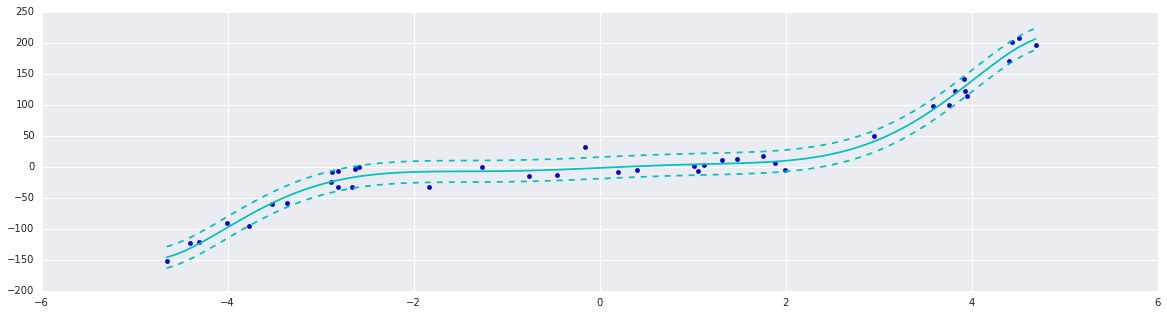
\includegraphics[scale=0.4]{no-linear}
\end{figure}

De esta forma, es directo ver que la fórmula del caso lineal es muy similar a este modelo, en donde cambiamos la variable \(t\) por la variable \(\phi(t)\), obteniendo así que la distribución predictiva de \(\bar{f}\) es normal con media y varianza
\begin{align*}
	p \left(\bar{f} \mid \bar{t}, T_n, \bfx_n\right)	&= \calN \left(\bar{\mu}_{\bar{f}}, \bar{\sigma}_{\bar{f}}^2\right),\\
	\bar{\mu}_{\bar{f}}									&= \bar{\phi} \left(\Phi_n^{\top} \Phi_n + \sigma^2 \Sigma_w^{-1}\right)^{-1} \Phi_n^{\top} \bfx_n,\\
	\bar{\sigma}_{\bar{f}}^2							&= \sigma^2 \bar{\phi} \left(\Phi_n^{\top} \Phi_n + \sigma^2 \Sigma_w^{-1} \right)^{-1} \bar{\phi}^{\top},\\
\end{align*}
donde \(\bar{\phi} = \phi(\bar{t})\) y \(\Phi_n = \phi(T_n)\).

\subsection{Modelo No Lineal No Paramétrico Bayesiano}

Es directo ver que para realizar predicciones utilizando este modelo es necesario invertir la matriz de tamaño \(\bar{d} \times \bar{d},\) la cual crece de forma cuadrática con respecto a la dimensión del espacio de características, volviéndose intratable si \(\bar{d}\) es muy grande.

Utilizando la formula de Woodbury, Sherman \& Morrison, el modelo puede reescribirse de una forma equivalente, pero que cambia por completo la interpretación del modelo, llevando el modelo paramétrico a su versión no paramétrica. Por simplicidad de notación, utilizaremos \(d\) como la dimensión del espacio de características. La versión de la fórmula que utilizaremos es
\[\left[Z + UWV^{\top}\right]^{-1} = Z^{-1} - Z^{-1} U^{\top} \left(W^{-1} + V^{\top} Z^{-1} U\right)^{-1} V Z^{-1},\]
con \(Z \in \reals^{d \times d}\), \(U, V\in \reals^{n\times d}\), y \(W \in \reals^{n\times n}\). Si aplicamos esta fórmula a la distribución predictiva de \(\bar{f}\), con \(Z = \sigma^2 \Sigma_w^{-1}\), \(U = V = \Phi_n\) y \(W = I_n\), entonces obtenemos que
\begin{align*}
	\left[Z + U W V^{\top}\right]^{-1}	&= \left[\sigma^2 \Sigma_w^{-1} + \Phi_n \Phi_n^{\top}\right]^{-1} \\
										&= \sigma^{-2} \Sigma_w - \sigma^{-2} \Sigma_w \Phi_n^{\top} \left[I_n + \Phi_n^{\top} \sigma^{-2} \Sigma_w \Phi_n\right]^{-1}\Phi_n \sigma^{-2} \Sigma_w \\
										&= \sigma^{-2} \Sigma_w \left(I_d - \Phi_n^{\top} \left[I_n + \Phi_n^{\top} \sigma^{-2} \Sigma_w \Phi_n\right]^{-1} \Phi_n \sigma^{-2} \Sigma_w \right) \\
	\bar{\phi} \left[\Phi_n^{\top} \Phi_n + \sigma^2 \Sigma_w^{-1} \right]^{-1} \Phi_n^{\top}	&= \sigma^{-2} \bar{\phi} \Sigma_w \left(\Phi_n^{\top} - \Phi_n^{\top} \left[I_n + \Phi_n^{\top} \sigma^{-2} \Sigma_w \Phi_n \right]^{-1} \Phi_n \sigma^{-2} \Sigma_w \Phi_n^{\top}\right) \\
																								&= \sigma^{-2} \bar{\phi} \Sigma_w \Phi_n^{\top} \left[I_n + \Phi_n^{\top} \sigma^{-2} \Sigma_w \Phi_n \right]^{-1} \\
																								&= \bar{\phi} \Sigma_w \Phi_n^{\top} \left[\sigma^2 I_n + \Phi_n^{\top} \Sigma_w \Phi_n \right]^{-1} \\
	\sigma^2 \bar{\phi} \left[\Phi_n^{\top} \Phi_n + \sigma^2 \Sigma_w^{-1}\right]^{-1} \Phi_n^{\top} \bar{\phi}	&= \bar{\phi} \Sigma_w \bar{\phi} - \bar{\phi} \Sigma_w \Phi_n^{\top} \left[\sigma^2 I_n + \Phi_n^{\top} \Sigma_w \Phi_n \right]^{-1} \Phi_n\Sigma_w\bar{\phi}.
\end{align*}
De esta forma, el modelo se puede reescribir como
\begin{align*}
	p \left(\bar{f} \mid \bar{t}, T_n, \bfx_n\right)	&= \calN \left(\bar{\mu}_{\bar{f}}, \bar{\sigma}_{\bar{f}}^2\right),\\
	\bar{\mu}_{\bar{f}}									&= \bar{\phi} \Sigma_w \Phi_n^{\top} \left[\sigma^2 I_n + \Phi_n^{\top} \Sigma_w \Phi_n \right]^{-1}\bfx_n,\\
	\bar{\sigma}_{\bar{f}}^2							&= \bar{\phi} \Sigma_w \bar{\phi}^{\top} - \bar{\phi} \Sigma_w \Phi_n^{\top} \left[\sigma^2 I_n + \Phi_n^{\top} \Sigma_w \Phi_n\right]^{-1} \Phi_n \Sigma_w \bar{\phi}^{\top}.
\end{align*}
Si denotamos \(K_n = \Phi_n^{\top} \Sigma_w \Phi_n\), \(\bar{k} = \bar{\phi} \Sigma_w \bar{\phi}^{\top}\) y \(\bar{\bfk}_n = \bar{\phi} \Sigma_w \Phi_n^{\top}\), lo anterior se simplifica a
\begin{align*}
	p \left(\bar{f} \mid \bar{t}, T_n, X_n\right)	&= \calN \left(\bar{\mu}_{\bar{f}}, \bar{\sigma}_{\bar{f}}^2\right), \\
	\bar{\mu}_{\bar{f}}								&= \bar{\bfk}_n^{\top} \left[K_n + \sigma^2 I_n\right]^{-1} \bfx_n, \\
	\bar{\sigma}_{\bar{f}}^2						&= \bar{k} - \bar{\bfk}_n^{\top} \left[K_n + \sigma^2 I_n\right]_n^{-1} \bar{\bfk}_n.
\end{align*}
Para realizar predicciones utilizando esta expresión, es necesario invertir la matriz \(K_n + \sigma^2 I_n\) de tamaño \(n \times n,\) que crece de forma cuadrática con respecto a la cantidad de observaciones (datos), independiente de la dimensión \(d\) del espacio de características, lo cual es más eficiente en el caso que \(d > n\).

\subsection{Modelo de Kernels Bayesiano}

Como podemos observar en la expresión final, todas las operaciones de los elementos del espacio de características tienen la forma de \(\phi(t_{1})^{\top} \Sigma_w \phi(t_{2})\), con \(t_{1}, t_{2} \in \calT\) y \(\phi(t_{1}), \phi(t_{2}) \in \calF\). Definiremos un \emph{kernel} como una función \(k : \calT \times \calT \to \reals\) de la siguiente forma:
\begin{equation*}
	k(t_{1}, t_{2}) = \phi(t_{1})^{\top} \Sigma_w \phi(t_{2}).
\end{equation*}


\begin{definition}
	Dado un conjunto de puntos \(T_n = \{t_{i}\}_{i=1}^n\) y un kernel \(k\) se define la matriz de Gram de \(k\) como aquella matriz \(K\) tal que \(K_{i,j} = k(t_{i}, t_{j})\).
\end{definition}

\begin{figure}[h]
	\centering
	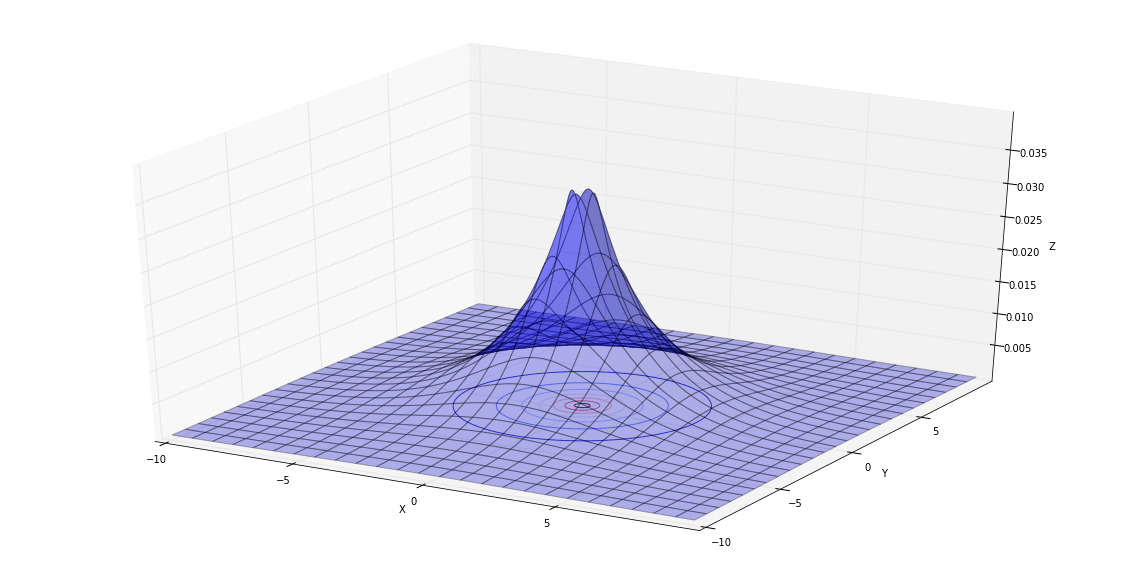
\includegraphics[scale=0.4]{kernel}
	\caption{Ejemplo de una función de kernel \(k : \calT \times \calT \to \reals\).}
\end{figure}
Podemos ver que \(\langle \phi_{1}, \phi_{2} \rangle_{\Sigma_w} = \phi_{1}^{\top} \Sigma_w \phi_{2}\) es un producto interno (con respecto a \(\Sigma_w\)) del espacio \(\calF\). Como \(\Sigma_w\) es definida positiva, se puede descomponer de forma que \(\Sigma_w = (\Sigma_w^{1/2})^{\top} \Sigma_w^{1/2}\). Por otro lado, si tomamos una descomposición en valores singulares de la matriz \(\Sigma_w = UDU^{\top}\), entonces \(\Sigma_w^{1/2} = UD^{1/2}U^{\top}\) cumple con la condición deseada. Con esto, es posible definir otra proyección
\begin{align*}
	\varphi : \calT	& \to \calF\\
	t						& \mapsto \varphi(t) = \Sigma_w^{1/2} \phi(t),
\end{align*}
de forma que el kernel \(k\) tiene forma de producto punto con respecto \(\varphi\), es decir,
\begin{align*}
	k(t_{1}, t_{2})	&= \left\langle \varphi(t_{1}), \varphi(t_{2}) \right\rangle\\
					&= \varphi(t_{1})^{\top} \varphi(t_{2})\\
					&= \phi(t_{1})^{\top} \Sigma_w \phi(t_{2}).
\end{align*}

Como la distribución posterior \(\bar{f} \mid \bar{t}, T_n, X_n\) está completamente definida en función de productos internos \(\phi(t_{1})^{\top} \Sigma_w \phi(t_{2})\), entonces es posible reemplazar dicha expresión por \(k(t_{1}, t_{2})\). Este reemplazo nos da la flexibilidad de modelar directamente el kernel \(k(t_{1}, t_{2})\), sin tener la necesidad de calcular \(\phi(t)\). Esta técnica se conoce como \emph{kernel trick}, y es útil cuando es más costoso calcular el vector de características que evaluar directamente el kernel, por ejemplo cuando la dimensión de características es infinita.

\section{Proceso Gaussiano}

Los modelos de regresión utilizando procesos gaussianos se pueden interpretar de dos formas diferentes. La primera se basa en que el kernel representa un producto interno en un espacio de gran dimensión (posiblemente infinita), y se realiza un modelo bayesiano lineal en dicho espacio. La segunda se basa en que la misma función de kernel representa la función de covarianza de un proceso estocástico, y que junto a la función de media determinan por completo el proceso gaussiano, que se puede pensar como una distribución sobre un espacio de funciones, donde la distribución predictiva se reescribe como
\begin{align*}
	p\left(\bar{f} \mid \bar{t}, T_n, \bfx_n\right)	&= \calN \left(\bar{\mu}_{\bar{f}}, \bar{\sigma}_{\bar{f}}^2\right),\\
	\bar{\mu}_{\bar{f}}								&= k(\bar{t}, T_n) \left[k(T_n, T_n) + \sigma^2 I_n\right]^{-1} \bfx_n,\\
	\bar{\sigma}_{\bar{f}}^2						&= k(\bar{t}, \bar{t}) - k(\bar{t}, T_n)^{\top} \left[k(T_n, T_n) + \sigma^2 I_n\right]^{-1} k(T_n, \bar{t}).
\end{align*}

Una de las formas más eficientes de calcular la media y la varianza posterior es utilizar la descomposición de Cholesky de la matriz \(k(T_n, T_n) + \sigma^2 I_n\), ya que los cálculos se reducen a calcular tres sistemas lineales, donde las matrices son triangulares, siendo muy eficientes y estables numéricamente.

A continuación se presenta un seudoalgoritmo para calcular la media y la esperanza posterior, además de la log-verosimilitud, utilizando la descomposición de Cholesky con el fin de ser más eficiente computacionalmente, y más estable numéricamente.

\begin{algorithm}
	\caption{Cálculo de media, varianza, y log-verosimilitud de un proceso gaussiano.}
	\begin{algorithmic}[1]
		\Require{\(T_n\) (inputs), \(\bfx_n\), (variables objetivo), \(k\) (kernel) \(\sigma^2\) (ruido) \(\bar{T}\) (\emph{inputs} de prueba).}
		\State \(L \gets\) la descomposición de Cholesky de \((k (T_n, T_n) + \sigma^2 I_n)\).
		\State \(\bfalpha \gets L^{\top} \backslash (L \backslash \bfx_n)\).
		\State \(\mean(f_{\ast}) \gets k (\bar{T}, T_n)^{\top} \bfalpha\).
		\State \(\bfv \gets L \backslash k(\bar{T}, T_n)\).
		\State \(\variance(f_{\ast}) \gets k(\bar{T}, \bar{T}) - \bfv^{\top} \bfv\).
		\State \(-\log \prob(\bfx_n \mid T_n) \gets \frac{1}{2} \bfx^{\top} \bfalpha + \sum_{i=1}^n \log(L_{ii}) + \frac{n}{2} \log(2\pi)\).
		\State \textbf{return} \(\mean(f_{\ast})\) (media), \(\variance(f_{\ast})\) (varianza), \(-\log \prob(\bfx_n \mid T_n)\) (log-verosimilitud negativa).
	\end{algorithmic}
\end{algorithm}

\begin{figure}[h]
	\centering
	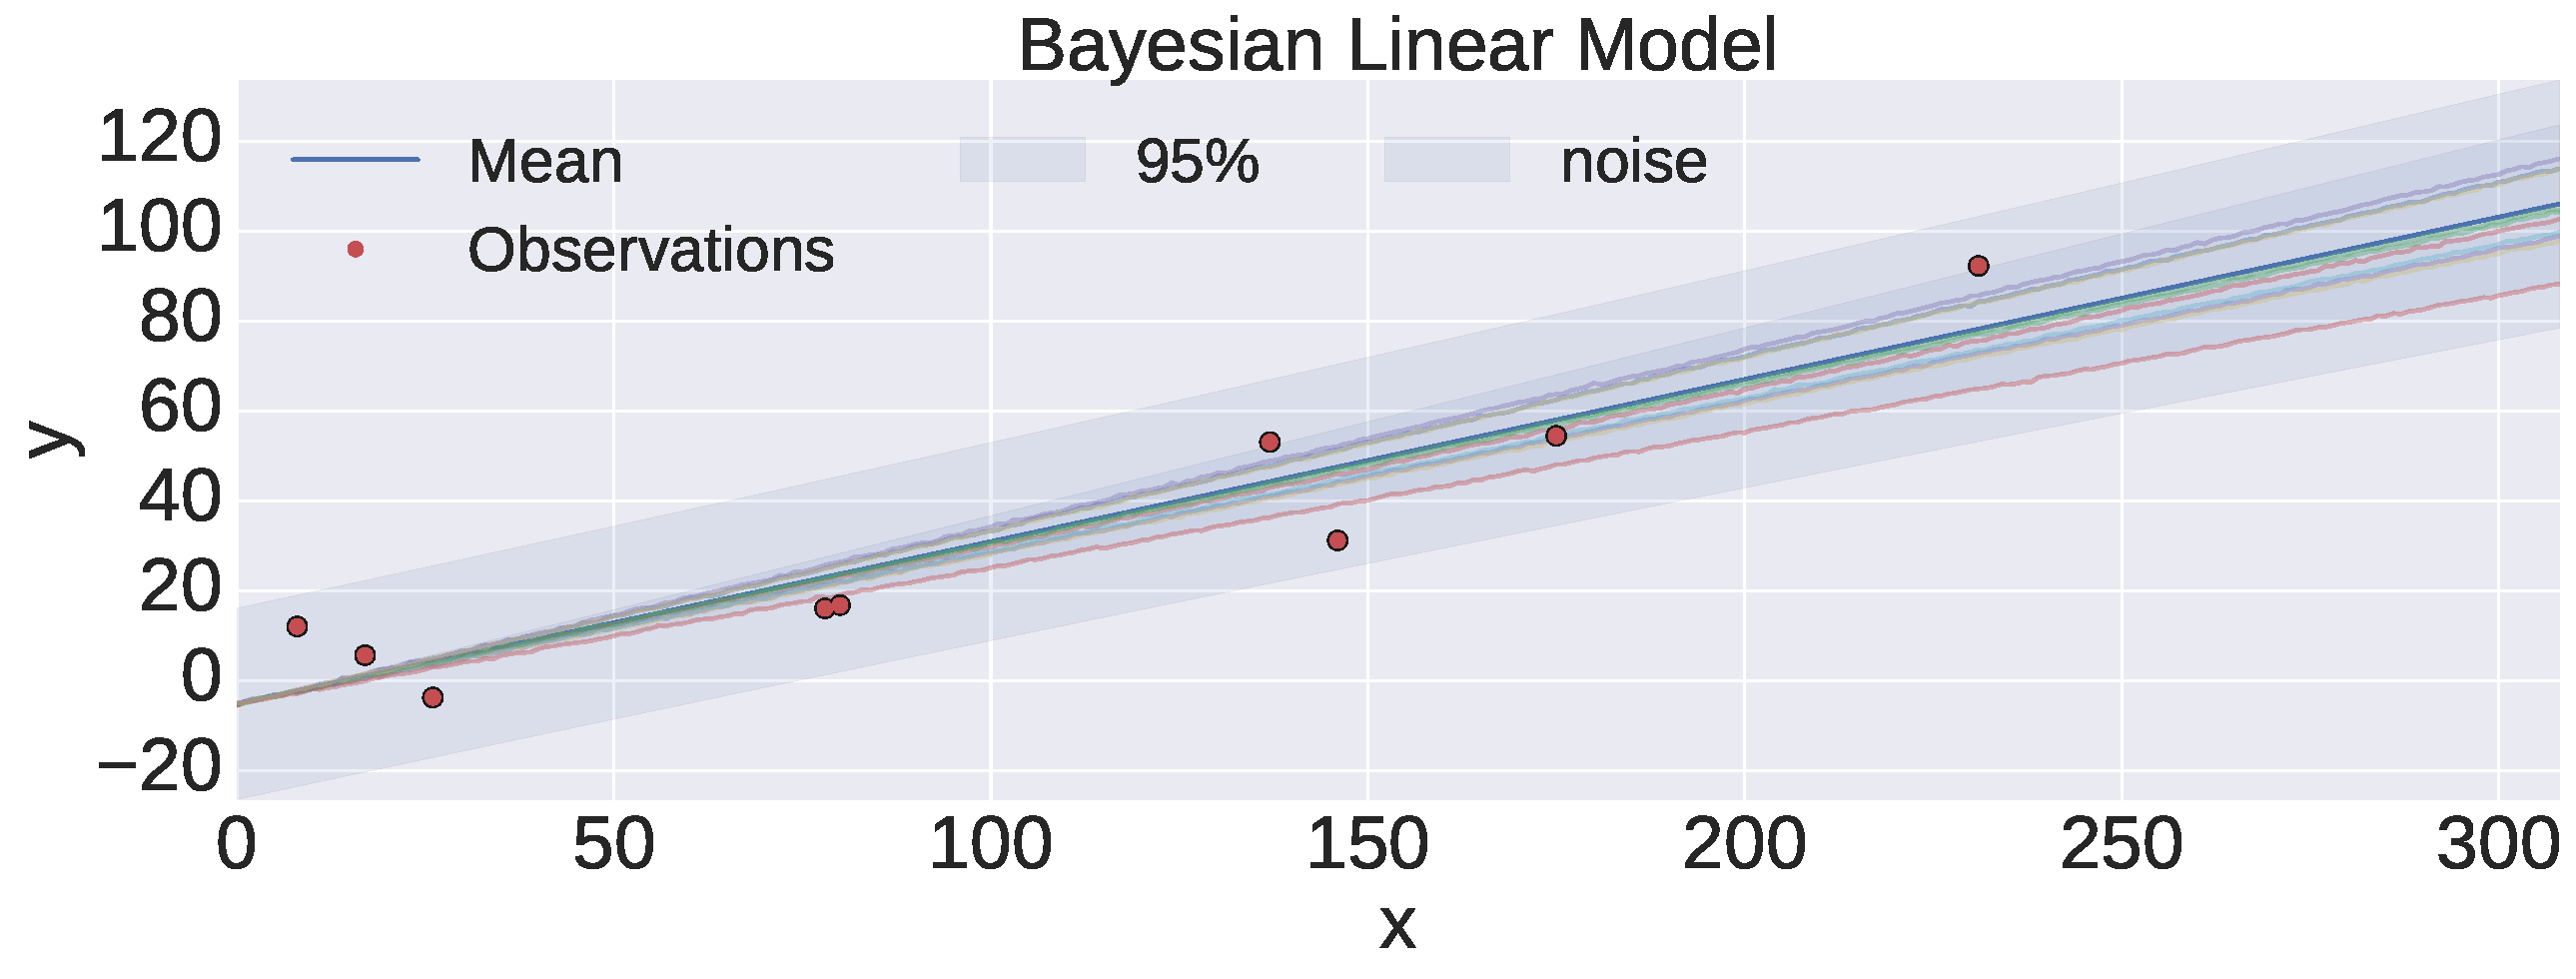
\includegraphics[width=0.49\textwidth]{bayesian_linear}
	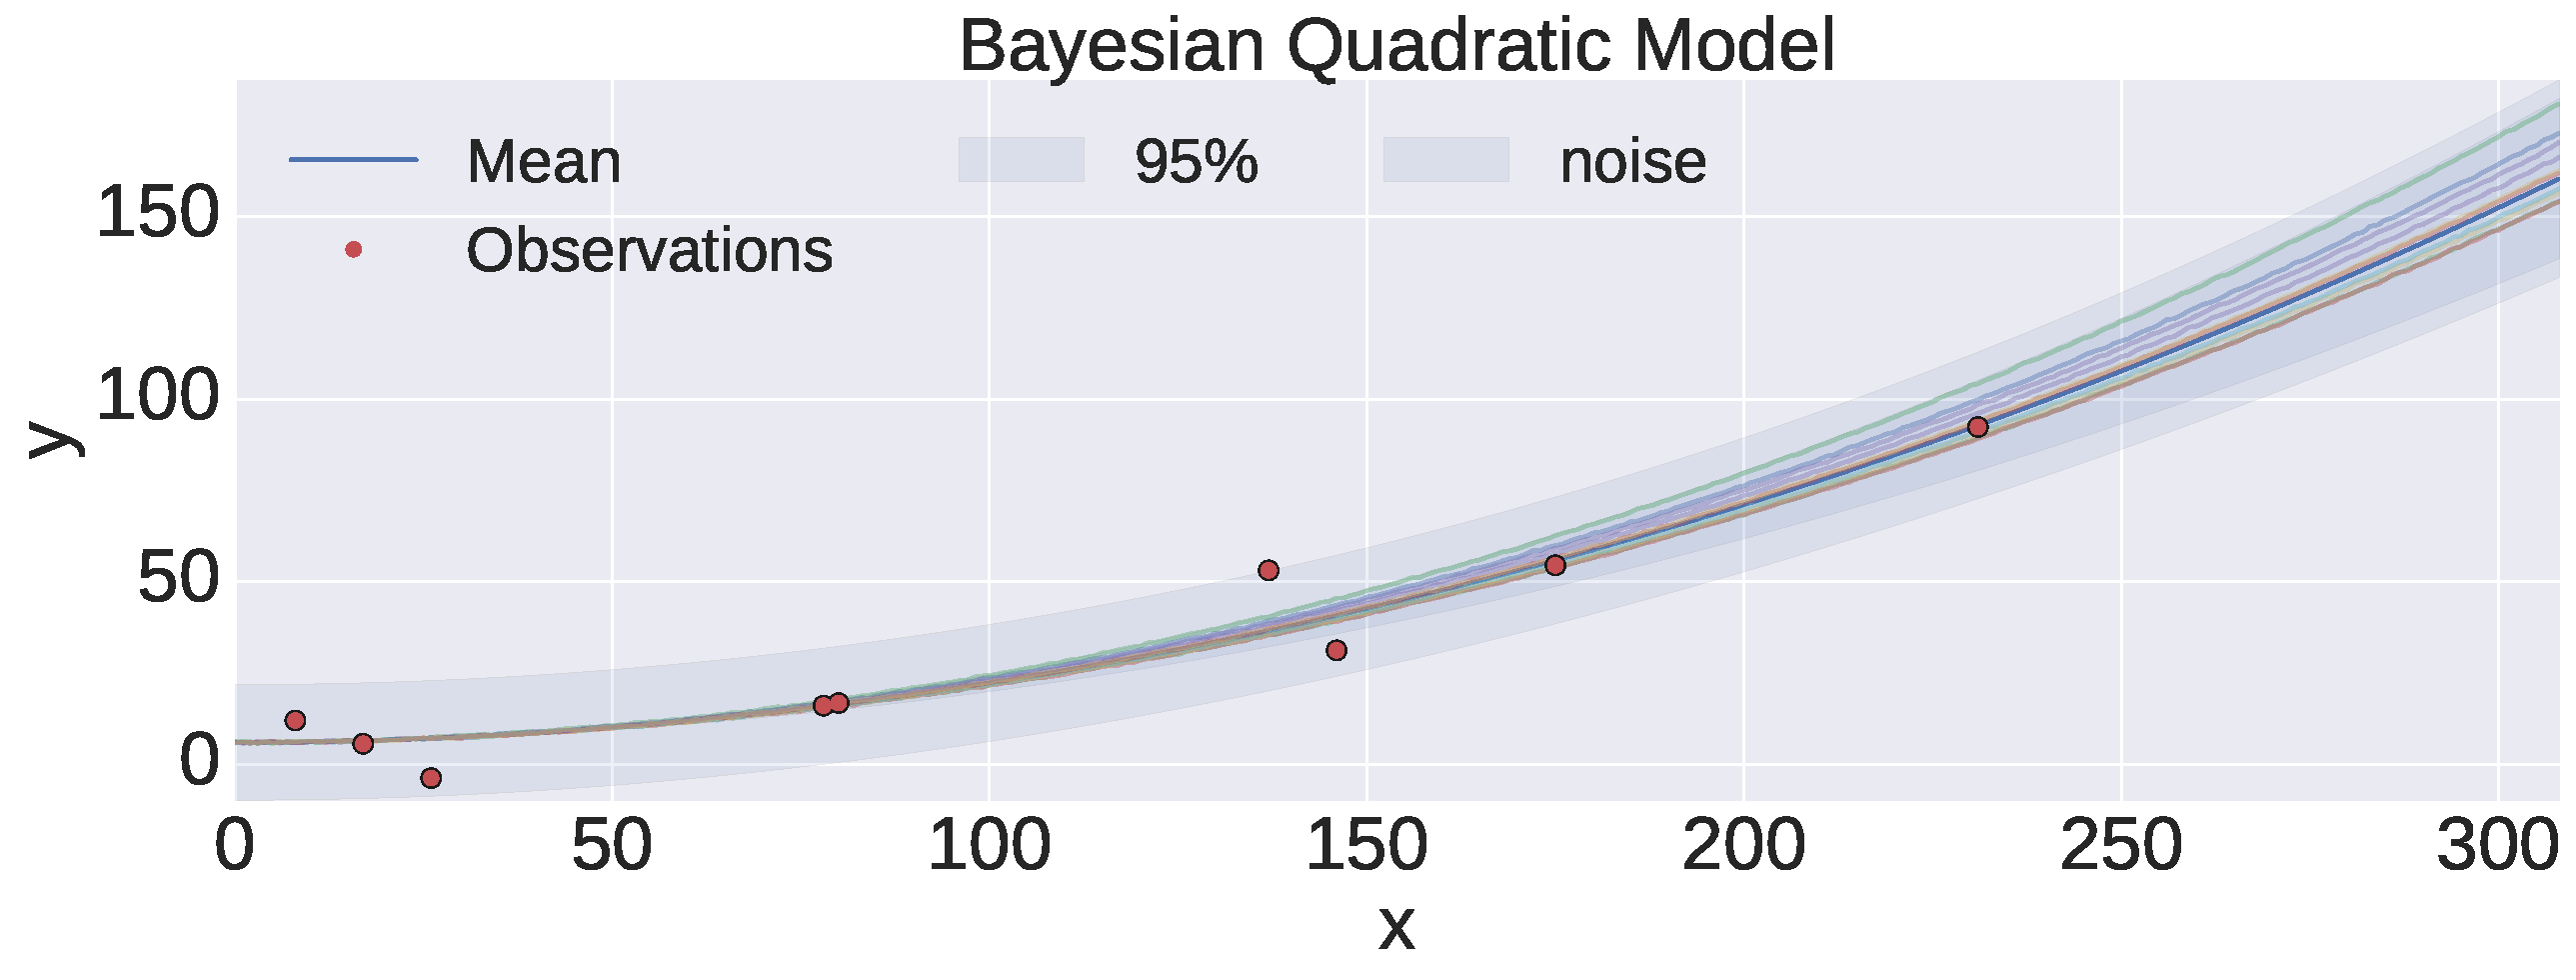
\includegraphics[width=0.49\textwidth]{bayesian_nonlinear}
	\caption{Izquierda: distribución posterior de un modelo lineal bayesiano. Derecha: distribución posterior de un modelo cuadrático bayesiano. Ambas posteriores consideran las mismas observaciones.}
	\label{fig:hierarchical_linear_quadratic}
\end{figure}

\subsection{De Redes Neuronales a Procesos Gaussianos}
\label{ssub:NN2GP}

\begin{figure}
	\centering
	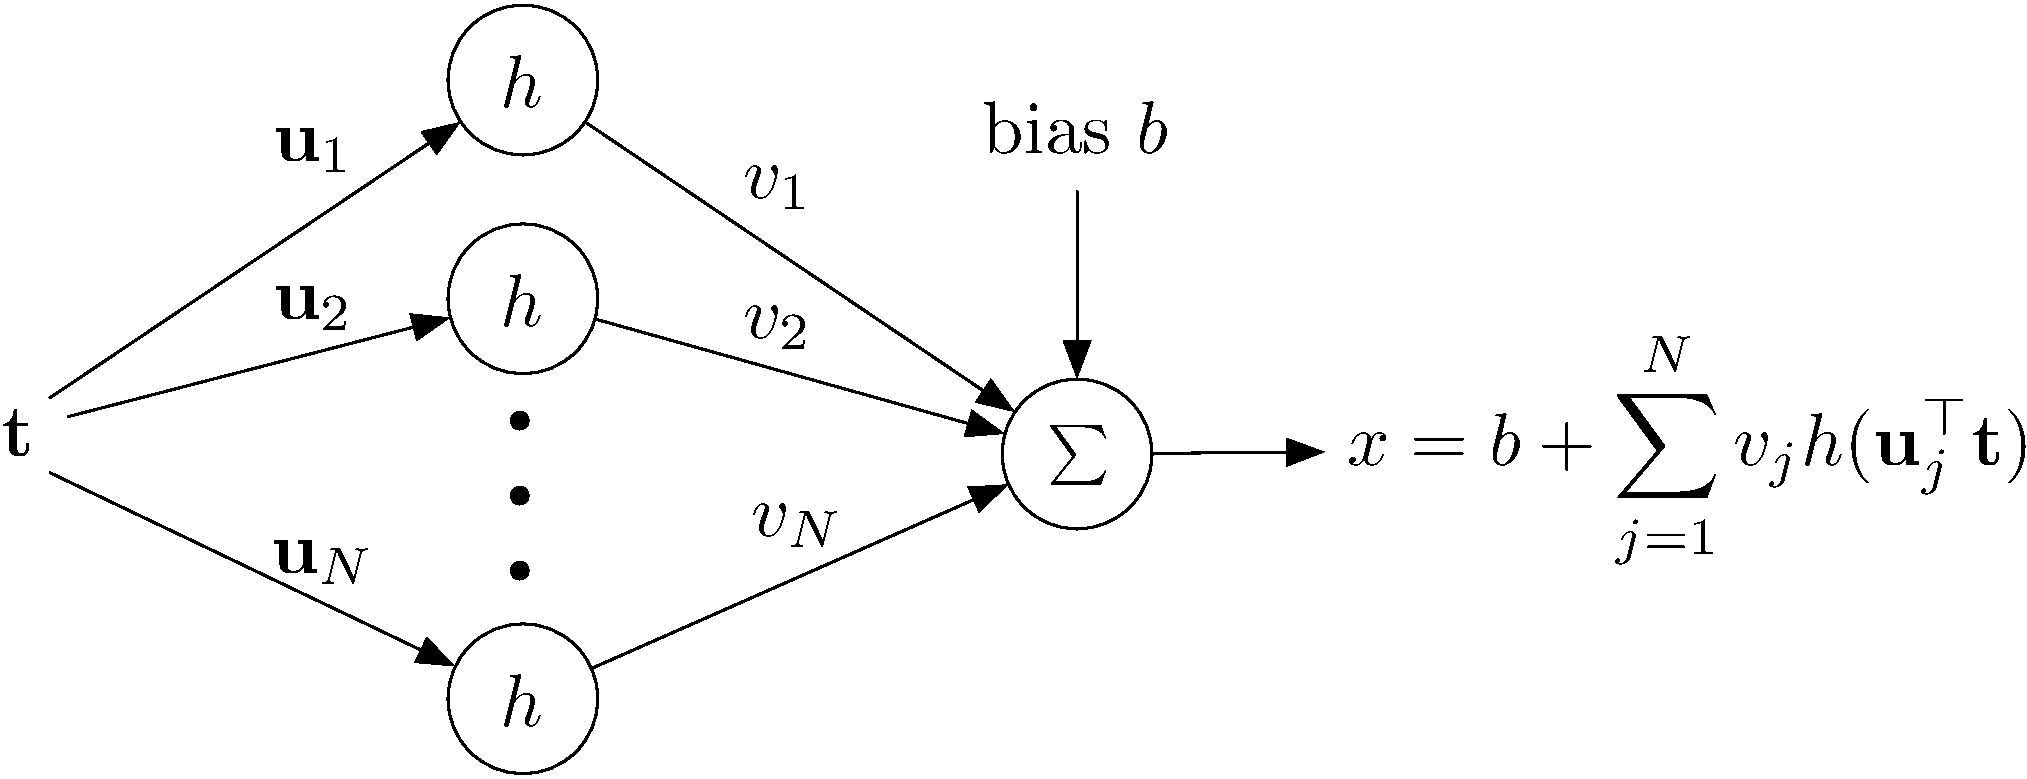
\includegraphics[width=0.5\textwidth]{nn}\\
	\caption{Red neuronal de una capa prealimentada: \(t\) es la entrada, \(x\) es la salida, \(h\) es la función de activación, \(b\) es el sesgo, \((\bfu_j)_{j=1}^N\) son los pesos de las entradas, \((\bfv_j)_{j=1}^N\) son los pesos de las salidas.}
	\label{fig:NN}
\end{figure}

Entre los practicantes de redes neuronales, se cree ampliamente que el número de neuronas debe ser determinada en base a la cantidad de datos disponible. Sin embargo, C. Williams señala en \cite{NIPS1996_1197} que esto tiene poco sentido desde un punto de vista bayesiano, en donde la complejidad del modelo se dicta por la complejidad del problema y no por la cantidad de datos disponible. En este sentido, R. Neal demostró que la salida de una red neuronal de una capa con pesos aleatorios converge a un proceso gaussiano cuando el número de neuronas tiende a infinito \cite{Neal:ARD}.

Siguiendo \cite{rasmussen06,NIPS1996_1197,Neal:ARD}, consideremos una red de \(n\) neuronas y una sola capa, como en la Figura \ref{fig:NN}. Al modelar el sesgo y los pesos como variables aleatorias independientes, las salidas \(x_1, x_2, \dotsc, x_n\) también son aleatorias para cualquier elección de entradas \(t_1, t_2, \dotsc, t_n\), con una distribución que no es necesariamente tratable debido a la función de activación no lineal \(h\). no obstante, notemos que la red en la Figura \ref{fig:NN} se define por una suma de términos i.i.d., por lo que en virtud del Teorema del Límite Central en múltiples dimensiones \cite{araujo1980central} hacer crecer el número de neuronas \(n \to \infty\) resulta en que las salidas \(x_1, x_2, \dotsc, x_n\) son conjuntamente gaussianas\footnote{La motivación de hacer crecer el número de neuronas a infinito se sigue de \cite{Hornik:1993}, que formula que la red de la Figura \ref{fig:NN} es un aproximador universal. Más aún, el TLC puede aplicarse pues como la función de activación \(h\) es acotada esto resulta en que las salidas \(x_1, x_2, \dotsc, x_n\) tienen varianza finita. Notemos que se requiere escalar la varianza de los pesos de salida proporcional a \(1/n\) para que se pueda aplicar el TLC.}. Esta construcción puede extenderse aún más al caso de un número infinito de entradas, lo que produce el proceso gaussiano \cite{rasmussen06}. En la siguiente sección profundizamos las propiedades de este modelo como un proceso estocástico.

\subsection{Distribución sobre Funciones}

Un enfoque alternativo de un proceso gaussiano consiste es describirlo como una distribución sobre funciones, donde la regresión corresponde a muestrear funciones, para luego calcular el promedio y la varianza del conjunto de funciones.
\begin{figure}[h]
	\centering
	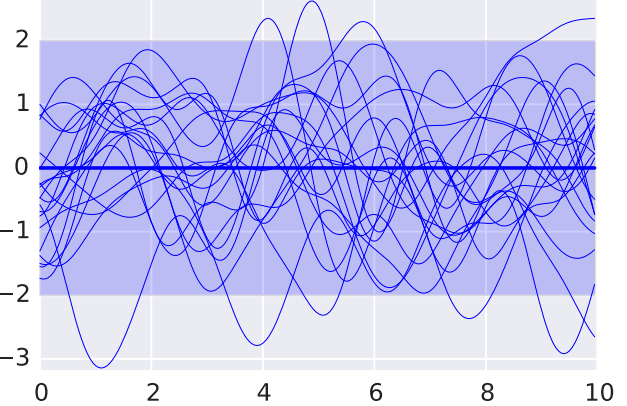
\includegraphics[scale=0.4]{gpdistribution}
	\caption{Representación gráfica de un proceso gaussiano, donde podemos distinguir su función de media, intervalos de confianza y muestras del proceso.}
\end{figure}

\begin{definition}
	Un \emph{proceso gaussiano} es una colección de variables aleatorias, donde todo subconjunto finito de ellas tiene distribución conjuntamente gaussiana.
\end{definition}

Un proceso gaussiano esta completamente especificado por su función de media \(m(t)\) y su función de covarianza \(k(t, t^{\prime})\), de forma que
\begin{align*}
	m(t)				&= \mean[f(t)],\\
	k(t, t^{\prime })	&= \mean[(f(t)-m(t))(f(t^{\prime })-m(t^{\prime}))^{\top}],
\end{align*}
y denotamos el proceso gaussiano como
\begin{equation*}
	f(t) \sim \GP(m(t), k(t, t^{\prime})).
\end{equation*}

La función de covarianza implica una distribución sobre funciones, por lo que para un conjunto de \(\no\) puntos de entrada \(\bar{T}\) podemos generar un vector aleatorio \(\bar{\bff}\) de forma que
\begin{equation*}
	\bar{\bff} \sim \calN(m(\bar{T}), k(\bar{T}, \bar{T})).
\end{equation*}

Para generar una muestra (o realización) del proceso, procedemos a calcular la descomposición de Cholesky de la matriz de covarianza \(k(\bar{T}, \bar{T})\), para luego construir una función lineal que, al evaluarla en un vector \(\bfu\) que distribuye conjuntamente como una normal unitaria, el resultado distribuye como el proceso gaussiano deseado. Esto se traduce en calcular \(L\) y simular \(\bfu\) de modo que
\begin{align*}
	k(\bar{T}, \bar{T})	&= LL^{\top},\\
	\bfu				&\sim \calN(\mathbf{0}, I_{\no}), \\
	\bar{\bff}			&= m(\bar{T}) + L\bfu.
\end{align*}

Consideremos el caso en el que las observaciones del proceso son sin ruido, es decir, \(\calD = \{(t_i, f_i)\}_{i=1}^n = \{T_n, \bff_n\}\). Sin perdida de generalidad, supongamos que nuestra función de media es
nula, es decir, \(m(t) = 0\). En efecto, en el caso general bastaría con redefinir nuestras observaciones como \(\hat{f}_i = f_i - m(t_i)\) y seguir con el análisis. Si deseamos conocer los valores \(\bar{\bff}\) que toma el proceso en \(\bar{T}\), entonces vemos que distribución conjunta de \(\bff_{n}\) y \(\bar{\bff}\) es
\begin{equation*}
	\begin{bmatrix}
		\bff_{n} \\
		\bar{\bff}
	\end{bmatrix}
	\sim \calN \left(\mathbf{0},
	\begin{bmatrix}
		k(T_n, T_n)		& k(T_n, \bar{T})\\
		k(\bar{T}, T_n)	& k(\bar{T}, \bar{T})
	\end{bmatrix}
	\right).
\end{equation*}
Luego, la distribución condicional de \(\bar{\bff}\) dados los datos \(\{T_n, \bff_{n}\}\) y el conjunto \(\bar{T}\) esta dada por
\begin{align*}
	p\left(\bar{\bff} \mid \bar{T}, T_n, \bff_{n}\right)	&= \calN\left(\bar{\mu}_{\bar{\bff}}, \bar{\sigma}_{\bar{\bff}}^2\right),\\
	\bar{\mu}_{\bar{\bff}}									&= k(\bar{T}, T_n) k(T_n, T_n)^{-1} \bff_{n},\\
	\bar{\sigma}_{\bar{\bff}}^2								&= k(\bar{T}, \bar{T}) - k(\bar{T}, T_n) k(T_n, T_n)^{-1} k(T_n, \bar{T}).
\end{align*}
La distribución condicional de cada punto \((t_i, f_i)\) dados los datos \(\{T_n, \bff_{n}\} \) está dada por \(p(f_i \mid t_i, T_n, \bff_{n}) = \calN(f_i, 0)\), lo que corresponde a una interpolación perfecta en los mismos puntos \((t_i, f_i)\), para \(i = 1, \dotsc, n\).

\subsection{Observaciones Ruidosas}

Consideremos ahora el caso más realista, en donde observamos el proceso más un ruido gaussiano, es decir \(\calD = \{(t_i,x_i)\}_{i=1}^n = \{T_n, \bfx_n\}\), donde \(x_i = f(t_i) + \varepsilon_i\) y los ruidos \(\varepsilon_i \sim \calN(0, \sigma^2)\) son independientes e idénticamente distribuidos. Siguiendo con el análisis anterior, y observando que \(\cov(x_i, y_j) = k(t_i, x_j) + \sigma^2 \delta_{ij}\), podemos ver que las probabilidades predictivas de \(\bar{\bff}\) e \(\bar{\bfx}\) están dadas por
\begin{align*}
	\begin{bmatrix}
		\bfx_n \\
		\bar{\bff}
	\end{bmatrix}
	&\sim \calN \left(\mathbf{0},
	\begin{bmatrix}
		k(T_n, T_n) + \sigma^2 I_n	& k(T_n, \bar{T})\\
		k(\bar{T}, T_n)				& k(\bar{T}, \bar{T})
	\end{bmatrix}
	\right), \\
	p\left(\bar{\bff} \mid \bar{T}, T_n, \bfx_n\right)	&= \calN\left(\bar{\mu}_{\bar{\bff}}, \bar{\sigma}_{\bar{\bff}}^2\right),\\
	p\left(\bar{\bfx} \mid \bar{T}, T_n, \bfx_n\right)	&= \calN\left(\bar{\mu}_{\bar{\bff}}, \bar{\sigma}_{\bar{\bff}}^2 + \sigma^2\right),\\
	\bar{\mu}_{\bar{\bff}}								&= \bar{\bfk}_{n}^{\top} \left[K_{n} + \sigma^2 I_n\right]^{-1}\bfx_n,\\
	\bar{\sigma}_{\bar{\bff}}^2							&= \bar{k}-\bar{\bfk}_{n}^{\top} \left[K_{n} + \sigma^2 I_n\right]^{-1} \bar{\bfk}_{n},\\
	K_{n}												&= k(T_n, T_n),\\
	\bar{\bfk}_{n}										&= k(T_n, \bar{T}),\\
	\bar{k}												&= k(\bar{T}, \bar{T}).
\end{align*}

Consideremos el caso en el que tenemos un único dato de entrada \(\bar{t}\). Podemos ver que \(\mean[\bar{f}] = \bar{\bfk}_{n} \left[K_{n} + \sigma^2 I_n\right]^{-1}\bfx_n\) es una combinación lineal de los \(n\) valores de \(\bfx_n\):
\begin{align*}
	\mean[\bar{f}]	&= \sum_{i=1}^{n} \alpha_i(\bar{t}) x_i\\
	\alpha(\bar{t})	&= \bar{\bfk}_{n}^{\top}(\bar{t}) \left[K_{n} + \sigma^2 I_n\right]^{-1},
\end{align*}
donde \(\alpha(\bar{t})\) se conoce como la \emph{función de peso} y es la representación de un suavizador linear, ya la predicción es una combinación lineal de las observaciones \(y\) suavizadas. Consideremos la descomposición en vectores propios de la matriz de covarianza:
\begin{equation*}
	K_{n} = \sum_{i=1}^{n} \lambda_i \bfu_i \bfu_i^{\top},
\end{equation*}
donde \(\lambda_i\) es su \(i\)-ésimo valor propio y \(\bfu_i\) es su correspondiente vector propio. Como \(K_{n}\) es real y simétrica semidefinida positiva, sus valores propios son reales y no negativos, y sus vectores propios son mutuamente ortogonales. Sea \(\bfx_n = \sum_{i=1}^{n} \gamma_i \bfu_i\) para coeficientes \(\gamma_i = \bfu_i^{\top} \bfx_n\). Entonces el vector de medias está dada por
\begin{align*}
	\mean[\bff_{n}]	&= K_{n} \left(K_{n} + \sigma^2 I_n\right)^{-1}\bfx_n \\
					&= \sum_{i=1}^{n} \frac{\gamma_i \lambda_i}{\lambda_i + \sigma^2} \bfu_i,
\end{align*}
donde el parámetro \(\sigma^2\) cumple el rol del nivel de suavizamiento.

A su vez, podemos ver que \(\mean[\bar{\bff}] = \bar{\bfk}_{n}^{\top} \left[K_{n} + \sigma^2 I_n\right]^{-1} \bfx_n\) es una combinación lineal de \(n\) funciones de kernels centradas en los puntos \(\bft_i\):
\begin{align*}
	\mean[\bar{\bff}]	&= \sum_{i=1}^{n} \beta_i k(t_i, \bar{t})\\
	\beta				&= \left[K_{n} + \sigma^2 I_n\right]^{-1} X_n.
\end{align*}%
Esta representación corresponde a un modelo lineal, ya que la predicción es una combinación lineal de funciones generadas por el kernel \(k(t, t^{\prime})\). Este kernel siempre existe, gracias al Teorema de Representación. Siempre y cuando \(k(t, t^{\prime})\) sea definido positivo, se dice que el kernel es una función de covarianza. En el próximo capítulo se realizará un análisis más formal de los kernel y sus espacios de funciones asociados.


\section{Entrenamiento de los Hiperparámetros}

En la sección anterior estudiamos como obtener la probabilidad predictiva, para utilizarla en la tarea de regresión. En todo momento se hizo la suposición que la función de kernel \(k(t, t^{\prime})\) estaba fija, pero en aprendizaje de máquinas deseamos encontrar el mejor modelo posible, lo que lleva a tener que encontrar el kernel y sus respectivos parámetros, que se conocen como hiperparámetros. En esta sección vamos a revisar cómo inferir los hiperparámetros para construir el modelo de regresión.

\subsection{Parametrización}
Aprender, dadas las observaciones \(\{T_n, \bfx_n\}\), es equivalente a encontrar funciones \(m\) y \(k\), usualmente parametrizadas por finitos parámetros \(\theta = (\theta_m, \theta_k) \in \reals^p\). Normalmente esto se logra vía la minimización de la la log-verosimilitud negativa, dada por
\[\ell \left(\theta\right) = \frac{n}{2}\log(2\pi) + \frac{1}{2} \left(\bfx_n - \mu \right)^{\top} K^{-1} \left(\bfx_n-\mu \right) + \frac{1}{2} \log \lvert K\rvert,\]
donde \(\mu\) y \(K\) son la media y la covarianza de \(\bfx_n\) dados los parámetros \(\theta = (\theta_m, \theta_k)\) y los inputs \(T_n\). Los métodos de optimización más usados son los basados en el gradiente, como el método BFGS de quasi-Newton, o métodos libre de derivadas como el método de Powell. En la Figura \ref{fig:gp_sunspots_example} mostramos un GP con un kernel \(\mathrm{SE}\) y con observaciones de actividad de manchas solares. El gráfico de la izquierda muestra el proceso con los hiperparámetros por defecto, mientras que el de la derecha tiene los hiperparámetros entrenados vía la log-verosimilitud negativa. En el segundo caso, la media está más cerca de la señar real (oculta), y el intervalo de confianza es más delgado, así que la predicción tiene menos incertidumbre.

Para la log-verosimilitud negativa donde la función de media es nula, la \(j\)-ésima componente del gradiente corresponde a la derivada parcial con respecto al parámetro \(\theta_j\) la cual se puede calcular como
\begin{align*}
	\pdv{\ell}{\theta_j}	&= \frac{1}{2}\bfx_n^{\top} K^{-1} \pdv{K}{\theta_j} K^{-1} \bfx_n + \frac{1}{2} \tr \left\vert K^{-1} \pdv{K}{\theta_j} \right\vert \\
							&= -\frac{1}{2} \tr\left(\left(K^{-1} \bfx_n \bfx_n^{\top} K^{-1} - K^{-1}\right) \pdv{K}{\theta_j}\right),
\end{align*}
donde \(\tr(A)\) denota la traza de la matriz \(A\).

La complejidad de computar la verosimilitud está dada por la inversión de la matriz \(K\), por lo que los métodos estándares de inversión de matrices simétricas definidas positivas de tamaño \(n \times n\) requieren tiempo \(O(n^{3})\). Una vez que la inversa está calculada, calcular la derivada requiere tiempo \(O(n^2)\) por cada hiperparámetro

\subsection{Seudoverosimilitud}

Los métodos de validación cruzada (\emph{cross-validation} en inglés) son métodos para seleccionar modelos. La idea más simple es la de dividir el conjunto de datos en dos conjuntos disjuntos: un conjunto de entrenamiento (\emph{training set} en inglés), el cual se utiliza para entrenar el modelo, y un conjunto de validación (\emph{validation set} en inglés), que se usa para medir el desempeño (o error) del modelo. Este método se conoce en inglés como \emph{holdout cross-validation}, y tiene el problema que si el conjunto de validación es pequeño, entonces la estimación del error tiene gran varianza.

Una alternativa es el método de validación cruzada en \(k\) iteraciones (\emph{k-fold cross-validation} en inglés), en done se divide el conjunto de datos en \(k\) conjuntos disjuntos de igual tamaño. Luego, cada conjunto es utilizado para validar y los otros \(k-1\) conjuntos son utilizados para entrenar, por lo que se realizan \(k\) entrenamientos y \(k\) estimaciones del desempeño, disminuyendo así la varianza de la estimación del error al tomar promedio. Un caso extremo es considerar \(k=n\). Esta validación cruzada dejando uno afuera (\emph{leave-one-out cross-validation} en inglés, y denotado denotado LOO más abajo) es utilizada sólo en casos particulares, por su alto costo computacional. En este caso, la log-probabilidad predictiva cuando se deja afuera el caso \(i\) es
\begin{align*}
	\log p(x_i \mid T_n, \bfx_{-i}, \theta)	&= -\frac{1}{2} \log (\sigma_i^2) - \frac{(x_i - \mu_i)^2}{2\sigma_i^2} - \frac{1}{2} \log(2\pi), \\
	\mu_i										&= K(t_i, T_{-i}) \left[K(T_{-i}, T_{-i}) + \sigma^2 I\right]^{-1} \bfx_{-i} \\
												&= x_i - \frac{[K^{-1} \bfx_n]_i}{[K^{-1}]_{ii}},\\
	\sigma_i^2								&= K(t_i, t_i) - K(t_i, T_{-i}) \left[K(T_{-i}, T_{-i}) + \sigma^2 I\right]^{-1} K(T_{-i}, t_i) \\
												&= \frac{1}{[K^{-1}]_{ii}} \\
	\log p(x_i \mid T_n, \bfx_{-i}, \theta)	&= \frac{1}{2}\log [K^{-1}]_{ii} - \frac{[K^{-1} \bfx_n]_i^2}{2 [K^{-1}]_{ii}} - \frac{1}{2} \log(2\pi),
\end{align*}
donde \(K = k(T_n, T_n)\), \(\bfx_{-i} = \bfx_n \setminus \{x_i\}\) y \(~T_{-i} = T_n \setminus \{t_i\}\). Luego, la log-probabilidad predictiva de LOO es
\begin{equation*}
	L_{LOO}(T_n, \bfx_n, \theta) = \sum_{i=1}^{n} \log p(x_i \mid T_n, \bfx_{-i}, \theta),
\end{equation*}
la cual se conoce como la seudo-log-verosimilitud (\emph{pseudo-log-likelihood} en inglés). Dada la inversa de \(K\), calcular \(L_{LOO}\) requiere tiempo \(O(n^2)\), y esta puede ser utilizada como estimador a optimizar con respecto a los hiperparámetros, quedando de la forma
\begin{equation*}
	L_{LOO}(T_n, \bfx_n, \theta) = -\frac{n}{2}\log(2\pi) + \frac{1}{2} \sum_{i=1}^{n} \left(\log [K^{-1}]_{ii} - \frac{[K^{-1} \bfx]_i^2}{[K^{-1}]_{ii}}\right).
\end{equation*}

Para calcular las derivadas parciales de \(L_{LOO}\) con respecto los hiperparámetros, veamos las derivas de las medias y las varianzas marginales.
\begin{align*}
	\pdv{\mu_i}{\theta_j}		&= -\pdv{\theta_j} \frac{\left[K^{-1} \bfx_n \right]_i}{[K^{-1}]_{ii}} \\
								&= \frac{\left[K^{-1} \pdv{K}{\theta_j} K^{-1} \bfx_{n}\right]_i [K^{-1}]_{ii} - \left[K^{-1} \bfx_n\right]_{ii} \left[K^{-1} \pdv{K}{\theta_j} K^{-1}\right]_{ii}}{[K^{-1}]_{ii}^2} \\
								&= \frac{\left[K^{-1} \pdv{K}{\theta_j} K^{-1} \bfx_{n}\right]_i}{[K^{-1}]_{ii}} - \frac{\left[K^{-1} \bfx_{n}\right]_{ii} \left[K^{-1} \pdv{K}{\theta_j} K^{-1}\right]_{ii}}{[K^{-1}]_{ii}^2}\\
	\pdv{\sigma_i^2}{\theta_j}	&= -\pdv{\theta_j} \frac{1}{[K^{-1}]_{ii}} \\
								&= \frac{\left[K^{-1} \pdv{K}{\theta_j} K^{-1}\right]_{ii}}{[K^{-1}]_{ii}^2}.
\end{align*}
Las derivadas con respecto a la media y la varianza de la log-probabilidad predictiva del \(i\)-ésimo término son
\begin{align*}
	\pdv{\mu_i} \log p(x_i \mid T_n, \bfx_{-i}, \theta)		&= \frac{x_i - \mu_i}{\sigma_i^2} = \left[K^{-1} \bfx_n \right]_i \\
	\pdv{\sigma_i^2}\log p(x_i \mid T_n, \bfx_{-i}, \theta)	&= \frac{(x_i - \mu_i)^2 - \sigma_i^2}{2 \sigma_i^4} = \frac{1}{2} \left[\left[K^{-1} \bfx_n\right]_i^2 - [K^{-1}]_{ii}\right].
\end{align*}
Luego, la derivada parcial de \(L_{LOO}\) con respecto al hiperparámetro \(\theta_j\) es
\begin{align*}
	\pdv{L_{\mathrm{LOO}}}{\theta_j}=	& \sum_{i=1}^{n} \pdv{\mu_i}{\theta_j} \pdv{\mu_i} \log p(x_i \mid T_n, \bfx_{-i}, \theta) + \pdv{\sigma_i^2}{\theta_j} \pdv{\sigma_i^2} \log p(x_i \mid T_n, \bfx_{-i}, \theta) \\
										=& \sum_{i=1}^{n} \frac{\left[K^{-1} \pdv{K}{\theta_j} K^{-1} \bfx_n \right]_i}{[K^{-1}]_{ii}} \left[K^{-1} \bfx_n\right]_i - \frac{\left[K^{-1} \bfx_n\right]_i \left[K^{-1} \pdv{K}{\theta_j} K^{-1}\right]_{ii}}{[K^{-1}]_{ii}^2} \left[K^{-1} \bfx_n\right]_i \\
										&+ \frac{\left[K^{-1} \pdv{K}{\theta_j} K^{-1}\right]_{ii} \left[\left[K^{-1} \bfx_n\right]_i^2 - \left[K^{-1}\right]_{ii}\right]}{2[K^{-1}]_{ii}^2} \\
										=& \sum_{i=1}^{n} \frac{\left[K^{-1} \bfx_n\right]_i}{\left[K^{-1}\right]_{ii}} \left[\left[K^{-1} \pdv{K}{\theta_j} K^{-1} \bfx_n\right]_i - \frac{[K^{-1}]_{ii} + \left[K^{-1} \bfx_n\right]_i^2}{2 \left[K^{-1} \bfx_n\right]_i[K^{-1}]_{ii}} \left[K^{-1} \pdv{K}{\theta_j} K^{-1}\right]_{ii}\right]
\end{align*}
Dada la inversa de \(K^{-1}\), la complejidad computacional de calcular una derivada parcial es de \(O(n^{3})\) por cada hiperparámetro, dominada por el término \(K^{-1} \pdv{K}{\theta_j} K^{-1}\). Mientras la función de verosimilitud marginal es la probabilidad de las observaciones dado el modelo, la función de seudoverosimilud es un estimador de la probabilidad predictiva del modelo.

\subsection{Selección de Variables}

Al momento de escoger un modelo, existe una gran variedad de familias de kernels (que se estudiarán en el próximo capítulo), donde cada una dispone de una cierta cantidad de hiperparámetros, los cuales deben ser entrenados (como vimos en las secciones anteriores), y esto depende fuertemente de la cantidad de variables que consideremos en el espacio de entrada, es decir de la dimensión \(d\) del espacio \(\calT\). El concepto de selección de modelo (\emph{model selection} en inglés) se refiere a la tarea general de escoger la familia de kernels, las variables de entrada y los hiperparámetros de un modelo.

En el caso que la dimensión \(d\) del espacio de entrada \(\calT\) sea mayor a uno, entonces los kernels deben permitir evaluar en todas las dimensiones. Puede darse el caso de que alguna de las dimensiones no afecte en la covarianza, ya sea porque la salida es independiente de esa dimensión o porque es redundante dada las demás dimensiones. En estos casos, reducir la dimensión del espacio \(\calT\) es deseable con el fin de bajar la complejidad del modelo. La opción más común es utilizar análisis de componentes principales (abreviado PCA pro sus siglas en inglés) sobre \(T_n\), pero este enfoque no es el más correcto, ya que no utiliza la información de \(\bfx_n\).

Consideremos el kernel \emph{square exponential}, dado por
\begin{equation*}
	k_{\mathrm{SE}} (t, \bar{t}) = h^2 \exp\left(-w^2 \left\Vert t - \bar{t} \right\Vert^2\right) = h^2 \exp\left(-w^2 \sum_{j=1}^{d} \left(t_j - \bar{t}_j\right)^2\right),
\end{equation*}
donde \(h\) y \(w\) son sus hiperparámetros. Se dice que este kernel es isotrópico, ya que todas las dimensiones de entrada son uniformes, supuesto que en muchos casos no es válido. La versión anisotrópica, conocida como \emph{automatic relevance determination} y denotada ARD, dada por
\begin{equation*}
	k(t, \bar{t}) = h^2 \exp\left(\sum_{j=1}^{d} w_d^2 (t_j - \bar{t}_j)^2\right),
\end{equation*}
tiene un hiperparámetro \(w_d^2\) por cada dimensión. Si \(w_d^2\) es muy pequeño o igual a \(0\), entonces se interpreta que la variable \(x_d\) no agrega información en la covarianza, por lo que son poco relevantes. Esto nos permite utilizar este kernel para eliminar variables poco relevantes. Una versión más sofisticada es el kernel de la forma
\begin{equation*}
	k(t, \bar{t}) = h^2 \exp\left(-\frac{1}{2} (t - \bar{t})^{\top} \left(\Lambda \Lambda^{\top} + \diag(w^2)\right) (t - \bar{t}) \right),
\end{equation*}
llamado la distancia del análisis de factor (\emph{factor analysis distance} en inglés), el cual generaliza el ARD con \(w = (w_1, \dotsc, w_D)\) y una matriz \(\Lambda\) de dimensión \(d \times k\), con \(k < d\). Además de determinar las relevancias individuales, las \(k\) columnas de \(\Lambda\) pueden identificar las direcciones que son más relevantes para explicar la varianza. Este kernel hace la analogía con el análisis factorial. Otro enfoque es considerar el kernel
\begin{equation*}
	k(t, \bar{t}) = \sum_{j=1}^{N} \frac{\phi_j(t) \phi_j(\bar{t})}{\alpha_j},
\end{equation*}
llamado máquina de relevancia vectorial (\emph{relevance vector machine} en inglés), donde \(\{\phi_j\}_{j=1}^{N}\) es una base de funciones. Este kernel permite reconocer las componentes \(\phi_j\) relevantes para explicar la covarianza, por lo que se pueden escoger las funciones base con diferentes conjuntos de variables de entrada, para así reconocer cuales son los conjuntos de variables más relevantes. Esta idea se puede extender con
\[k (t, \bar{t}) = \sum_{j=1}^{N} \frac{k_j(t, \bar{t})}{\alpha_j}.\]